\chapter{总结与展望}\label{chp:summary}
\section{工作归纳}
本文在信息论度量应用到社团发现领域的已有工作基础上,
从普适信息论和随机图建模两种思路入手,
建立了信息论度量和社团发现问题在理论分析和算法设计两个层面的联系。
具体来说,本文的工作可总结为以下三部分:

首先,在社团的层次化发现问题上,我们基于多变量互信息对层次化发现问题
进行理论建模,证明了弱独立的随机变量的多变量互信息的计算可以化为一个社团发现问题,
并由此提出了用聚类树表示的层次化结构,与已有的主分割序列PSP算法建立了联系。
进一步地,我们提出了一种高效的层次化发现计算策略——HPSP算法,
该算法的时间复杂度比求解主分割序列的现有算法低一个数量级,
使得应用多变量互信息在中等规模的网络中进行社团层次化发现成为可能。
我们利用多变量互信息的理论,也对异常值检测问题进行了相关的算法设计和实验验证。
该异常值检测算法在未知异常值点数量、含有多个类别的数据集问题上具有应用的潜力。

其次,在统计物理启发的社团发现算法方面,我们采用了随机块模型对网络进行建模,
研究了玻茨模型达到精确恢复的条件。我们的结果表明,玻茨模型在随机块模型的社团发现
问题中存在相变现象,在可达到精确恢复的区域内,我们给出了算法误差衰减速率的上界。
进一步地,我们揭示了基于玻茨模型的算法与能量最小化算法、最小割算法、
最大似然算法、最大模块度算法的联系,并比较了它们的误差衰减速率的上界。
该方面的研究为算法分析提供了统一的分析框架,给出了相关算法误差率的理论保证。

最后,在有辅助信息的社团发现问题上,我们基于雷尼散度研究了有辅助信息的随机块模型,
给出了该模型下实现精确恢复的充要条件,并推导了最优误差衰减率的理论极限。
该结果定量地刻画了节点辅助信息和边信息各自对恢复问题的贡献,
对于指导辅助信息采样数量的选取具有重要意义。
在此基础上,我们设计了半正定规划算法,可满足精确恢复的要求。
在不同参数设定下的实验结果进一步验证了半正定规划算法在有辅助信息的社团发现问题上的有效性。

%本文的工作在社团发现领域具有重要的应用价值。
   %\begin{figure}[!ht]
%    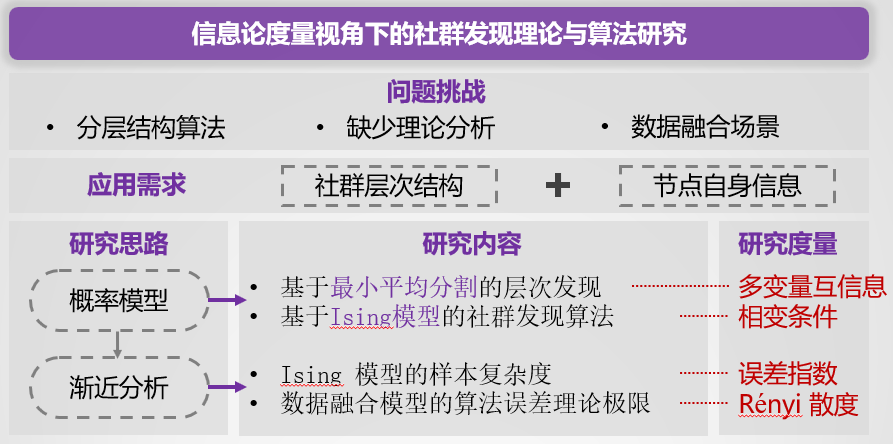
\includegraphics[width=0.9\linewidth]{screenshot-20230130-193759.png}
%\end{figure}

\section{分析技术评注}
本文综合运用了多种信息论
度量研究社团发现问题。
它们均是针对
概率分布的距离度量,可总结为下表:
\begin{table}[!ht]
    \centering
  \begin{tabular}{ccp{5cm}}
    \hline
     度量名称    &   参数个数 &   本文所处理的分布 \\
    \hline
     多变量互信息 &    $\geq 2$ &    弱独立的随机变量  \\
     速率函数     &    1 &     两个二项分布的差  \\
     雷尼散度     &    2 &    泊松分布和字母集有限的离散型随机变量 \\
    \hline
  \end{tabular}
  \caption{各种信息论度量的对象}\label{tab:info_metric}
\end{table}

除以上信息论度量外,本文还综合运用了在信息论与统计学的交叉研究领域中的大偏差理论和假设检验问题的研究成果。
在技术证明中,用到了分治算法分析、优化中的对偶理论以及概率论中的相关结论。

信息论度量的分析方法有赖于相关假设的引入,比如
随机变量弱独立、网络由对称的随机块模型生成等假设。这些假设
本质上是数学中无穷小、无穷大量的具体实例,引入它们的目的是为了
考察算法或模型的渐近性质。需要指出的是,实际网络中节点往往不满足
弱独立的假设,网络结构也与随机块模型的统计特征不尽相同,但这并
不影响基于信息论度量分析方法本身的重要性和有效性。

\section{研究展望}
本文的研究可在多方面进行拓展。

在算法设计层面,由于实际处理的图的规模可能比较大,
仿照 \citet{faysal2021parallel} 中对 Infomap 这一社团发现算法并行化的思路,
我们可以考虑本文所研究的HPSP算法,梅特罗波利斯算法的并行化。
而在研究玻茨模型的相变性质层面,我们可以从分布
\eqref{eq:isingma}独立采集多个
样本,通过系综学习(如多数同意规则)的方式进行社团发现,
然后研究相变点$\beta$和样本数的关系。

此外,本文研究的是带有辅助信息的两社团随机块模型,
该研究思路有望拓展到其他随机图模型或多社团随机块模型上,并
通过似然函数构建类似\eqref{eq:matrix_mle}式
的优化目标,从而指导
一般性的有辅助信息的图模型的
算法设计。然后我们可以将该方法与通过其他准则\cite{chunaev2020community}构建的算法进行
比较探索其适用场景。

另一方面,随着深度学习技术的兴起,社团发现任务亦可由
神经网络模型藉以完成,尤其是在有辅助信息的场景下 \cite{cao2018incorporating}。
仿照本文研究梅特罗波利斯算法、半正定方法的思路,
未来可研究神经网络模型在随机块模型上的恢复误差,即可解释性问题。